\documentclass[lecture.tex]{subfiles}

\begin{document}

\exercice{Jessy Lefeuve}
%\video{https://youtu.be/blablabla}
\enonce{rdm-0025}{Etude du Golden Gate}

Le Golden Gate de San Francisco est soumis à de nombreuses sollicitations. Nous nous proposons de réaliser une étude pour deux cas chargement distincts. Ces deux cas pourront être étudiés indépendamment l’un de l’autre. Les deux parties de l’exercice sont indépendantes.

\begin{center}
  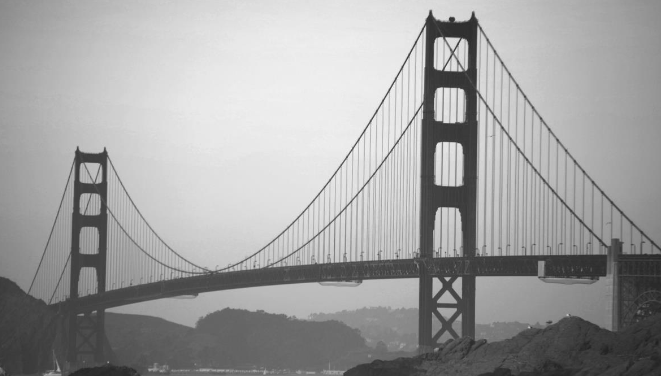
\includegraphics[scale=0.4]{figA0025.png}
\end{center}

En première approximation, le pont du Golden Gate peut être modélisé de la façon suivante, en négligeant les efforts de pesanteur.

\begin{center}
  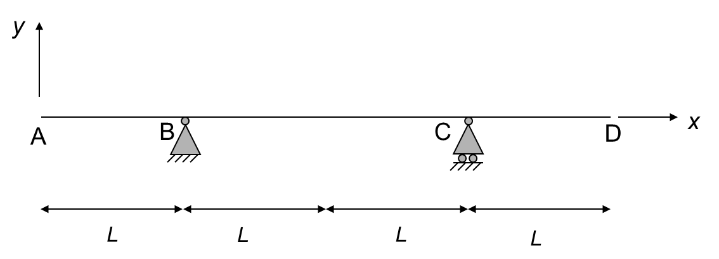
\includegraphics[scale=0.4]{figB0025.png}
\end{center}

Au point B, le pont est lié à une liaison rotule (ou pivot). Au point C, la liaison est modélisée par un appui ponctuel (ou pivot glissant).

\bigskip

\begin{description}
  \item[Première partie : Pont soumis à une charge ponctuelle] \ \par
  %
  Un poids lourd s’engage sur le pont au point A. Il est modélisé par un effort $F$ orienté selon l’axe $-y$ comme illustré sur le schéma ci-dessous.
  \begin{center}
    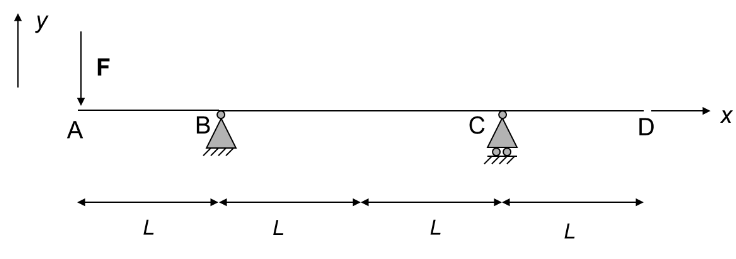
\includegraphics[scale=0.4]{figC0025.png}
  \end{center}
  \begin{enumerate}
    \item Démontrez l'isostaticité de la structure.
    \item Déterminez les expressions des inconnues de liaisons par application du Principe Fondamental de la Statique (PFS).
    \item Après avoir précisé les inconnues de liaisons non nulles sur un schéma, déterminez le nombre de coupures nécessaires au calcul des efforts internes et les expressions des efforts internes à la structure $N$, $T$ et $M$ en fonction de l'abscisse $x$ pour chaque coupure.
    \item Tracer les diagrammes des efforts internes dans le cas suivant, sur les schémas ci-dessous. On donne $F = 400 \ kN$ et $L = 300 \ m$.
  \end{enumerate}
  %
  %
  \item[Deuxième partie : Pont soumis à deux types de charge] \ \par
  %
  Le poids lourd tombe en panne au milieu du pont (point E ci-dessous). Un embouteillage se forme entre le point A et le point E. Les efforts engendrés par les véhicules à l’arrêt sont modélisés par une charge répartie $p$ orientée vers l’axe $-y$. Le poids lourd est modélisé par l’effort ponctuel $F$ au point E orienté vers le bas $-y$. Le schéma suivant représente le problème à étudier.
  \begin{center}
    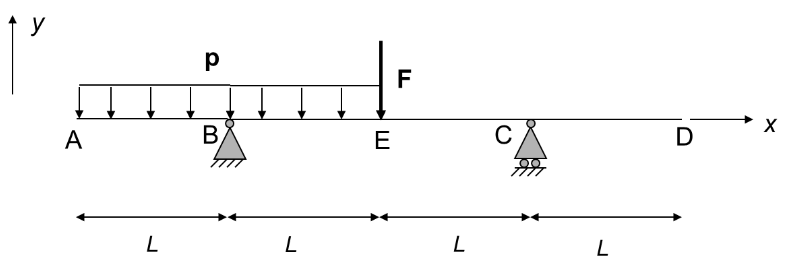
\includegraphics[scale=0.4]{figD0025.png}
  \end{center}
  \begin{enumerate}
    \item Déterminer les réactions aux appuis en B et en C.
    \item Déterminer le nombre de coupures nécessaires à la détermination des efforts internes sur l’ensemble de la structure, puis déterminer ces efforts internes $N$, $T$ et $M$ tout au long de la poutre.
    \item Tracer les trois diagrammes des efforts internes tout au long de la poutre dans le cas suivant. On donne $F = 400 \ kN$, $p = 3000 \ kN/m$ et $L = 300 \ m$.
  \end{enumerate}
  %
\end{description}

\finenonce{rdm-0025}
\finexercice


\end{document}
